\documentclass[a4paper]{article}
\usepackage[utf8]{inputenc}
\usepackage[russian,english]{babel}
\usepackage[T2A]{fontenc}
\usepackage[left=10mm, top=20mm, right=18mm, bottom=15mm, footskip=10mm]{geometry}
\usepackage{indentfirst}
\usepackage{amsmath,amssymb}
\usepackage[italicdiff]{physics}
\usepackage{graphicx}
\usepackage{multirow}
\usepackage{svg}
\graphicspath{{images/}}
\DeclareGraphicsExtensions{.pdf,.png,.jpg}
\usepackage{wrapfig}
\usepackage{caption}
\captionsetup[figure]{name=Рисунок}
\captionsetup[table]{name=Таблица}
\title{\underline{Длинная Линия}}
\author{Каспаров Николай, Б01-304}

\begin{document}

\maketitle
\begin{center}
\Large{\textbf{ }}
\end{center}

\subparagraph{Цель работы:}

    Ознакомится и проверить на практике теорию распространения
    электрических сигналов вдоль длинной линии; измерить амплитудо- и фазово-частотные
    характеристики коаксиальной линии; определить погонные характеристики такой
    линии; на примере модели длинной линии изучить вопрос распределения амплитуды
    колебаний сигнала по длине линии.

\subparagraph{В работе используются:}

    Осциллограф; генератор сигналов; коаксиальный кабель; схематический блок "модель длинной линии"; магазин
    сопротивления Р33, соединительные провода.

\section{Ход работы}

\subsection{Определение параметров коаксиального кабеля}

Для определения характеристик коаксиального кабеля
удобно записать следующее уравнение:

\begin{equation}
    y_1 = \frac{L_x C_x}{c^2}x_1, 
\end{equation}
где

\begin{equation}
    x_1 = \omega^2
\end{equation}

\begin{equation}
    y_1 = k(\omega)^2 - \alpha (\omega)^2
\end{equation}

Занесем данные в таблицу:

\begin{figure}[h!]
    \centering
    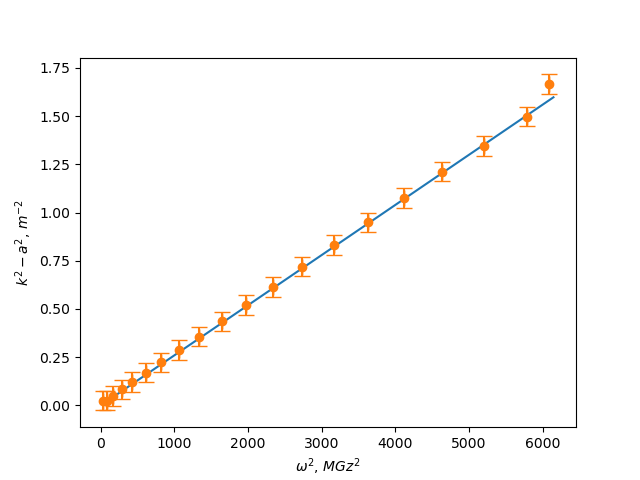
\includegraphics[width=0.6\pdfpagewidth]{graph1.png}
    \caption{Определение параметров коаксиального кабеля}
\end{figure}

Отсюда найдем $L_xC_x$:

\begin{equation}
    \beta = L_xC_x = (2.34 \pm 0.02)
\end{equation}

Т.к. линия согласована:
\begin{equation}
    L_x = cR_0 \cdot \sqrt{\beta} = (2.55 \pm 0.03)
\end{equation}
\begin{equation}
    C_x = \sqrt{\beta} / cR_0 = (0.92 \pm 0.01)
\end{equation}

Также для коаксиального каебля верно:

\begin{equation}
    L_x = 2 \mu \ln(r_2/r_1)
\end{equation}
\begin{equation}
    C_x = \frac{\varepsilon}{2 \ln(r_2/r_1)}
\end{equation}

Отсюда получаем:

\begin{equation}
    \mu = \frac{L_x}{2 \ln(r_2/r_1)} = (1.13 \pm 0.01)
\end{equation}
\begin{equation}
    \varepsilon = 2 \ln(r_2/r_1) \cdot C_x = (2.06 \pm 0.02)
\end{equation}

\subsection{Оценка фазовой скорости}

Подадим синусоидальный сигнал на длинную линию и будем регистрировать резонансные частоты.

\begin{equation}
    k = \frac{2\pi (n + n_0)}{l},
\end{equation}
или через фазовую скорость:


\begin{equation}
    \nu_n = \frac{V_\phi}{l} (n + n_0)
\end{equation}

\begin{figure}[h!]
    \centering
    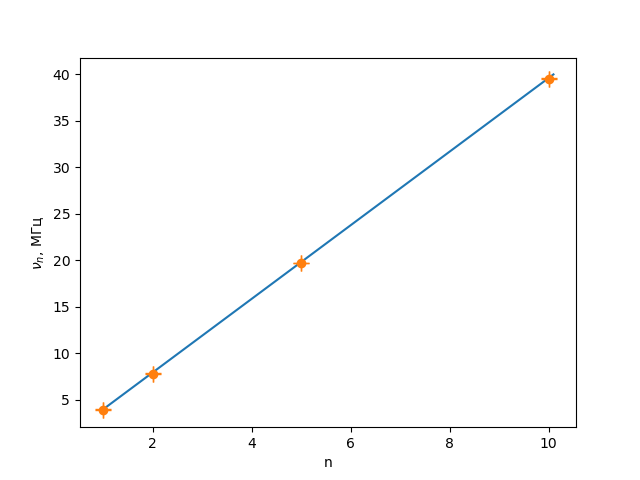
\includegraphics[width=0.6\pdfpagewidth]{graph2.png}
    \caption{Оценка фазовой скорости}
\end{figure}

Полученный коэффициент наклона:

\begin{equation}
    \frac{V_\phi}{l} = (3.958 \pm 0.004) ~ \text{МГц},
\end{equation}
отсюда

\begin{equation}
    V_\phi = (1.98 \pm 0.01) \cdot 10^{10} ~ \frac{\text{см}}{\text{с}}
\end{equation}

\subsection{Определение удельной проводимости проводников. Метод А}

Имеем соотношение

\begin{equation}
    \alpha = \frac{4}{\sqrt{\sigma}d}C_x\frac{V_\phi}{c}\sqrt{\nu} + \alpha_0
\end{equation}

Построим зависимость $y_2(x_2)$, где $y_2 = \alpha$, а $x_2 = \sqrt{\nu}$,
отсюда:

\begin{equation}
    \sigma_1 = \left( \frac{4C_xV_\phi}{cd \left( \frac{\Delta y}{\Delta x} \right)} \right)^2
\end{equation}

\begin{figure}[h!]
    \centering
    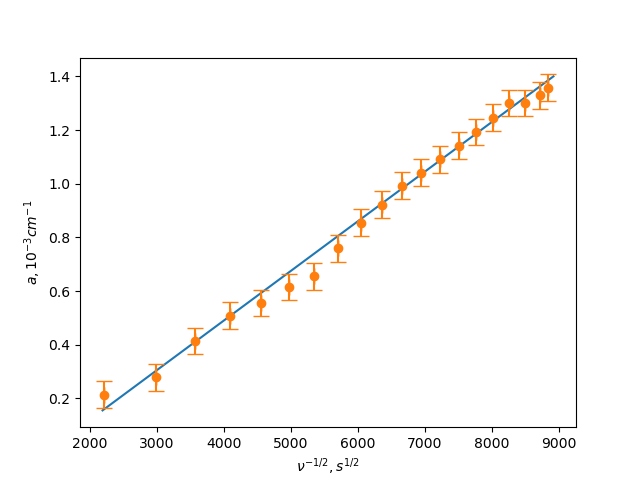
\includegraphics[width=0.6\pdfpagewidth]{graph3.png}
    \caption{Метод А}
\end{figure}

Отсюда имеем:

\begin{equation}
    \sigma_1 = (5.4 \pm 0.1) \cdot 10^{18}
\end{equation}

\subsection{Определение удельной проводимости проводников. Метод Б}

Для данного метода построим зависимость $\alpha k$ от $\nu^{3/2}$:

\begin{equation}
    y_3 = \frac{4\pi C_x}{cd\sqrt{\sigma}}x_3
\end{equation}

Отсюда 
\begin{equation}
    \sigma_2 = \left( \frac{4\pi C_x}{cd \left( \frac{\Delta y}{\Delta x}\right)} \right)^2 = (6.7 \pm 0.3) \cdot 10^18
\end{equation}

\begin{figure}[h!]
    \centering
    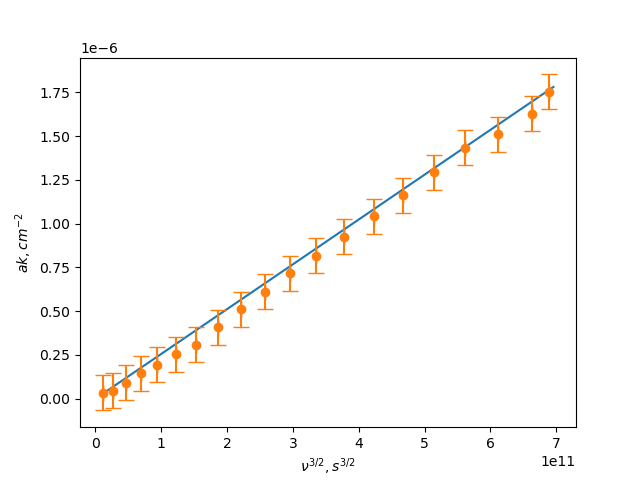
\includegraphics[width=0.6\pdfpagewidth]{graph4.png}
    \caption{Метод Б}
\end{figure}

\section{Вывод}

В ходе данной работы была изучена теория распространения электрических сигналов вдоль длинной линии, а также экспериментально проверены её основные положения. Измерены амплитудно- и фазово-частотные характеристики коаксиальной линии, определены её погонные параметры: индуктивность $L_x = (2.55 \pm 0.03)$, емкость $C_x = (0.92 \pm 0.01)$, а также магнитная проницаемость $\mu = (1.13 \pm 0.01)$ и диэлектрическая проницаемость $\varepsilon = (2.06 \pm 0.02)$ диэлектрика. Оценена фазовая скорость распространения сигнала в линии $V_\phi = (1.98 \pm 0.01) \cdot 10^{10}$ см/с.

Двумя различными методами (А и Б) определена удельная проводимость проводников коаксиального кабеля. Метод А дал значение $\sigma_1 = (5.4 \pm 0.1) \cdot 10^{18}$, в то время как метод Б показал $\sigma_2 = (6.7 \pm 0.3) \cdot 10^18 $.

Таким образом, работа позволила на практике изучить теорию длинной линии, исследовать её характеристики и проверить экспериментальные методы измерения параметров электрических цепей.

\end{document}
